% !TEX program  = pdflatex --shell-escape

\documentclass[12pt]{article}

\usepackage{natbib}
\usepackage{times}
\usepackage[T1]{fontenc}
\usepackage[utf8]{inputenc}
\usepackage[pdftex]{graphicx}
\usepackage[letterpaper, left=1.0in, right=1.0in, top=1in, bottom=1in]{geometry}

\usepackage{ragged2e}
\usepackage{upquote}

\usepackage[backref=page]{hyperref}
\usepackage{hyperref}
\usepackage{rotating}
\usepackage{booktabs}
\usepackage[hypcap, labelsep=period]{caption}
\usepackage{array}
\usepackage{color}
\usepackage{newfloat}
\usepackage{url}
\usepackage{bm}
\usepackage{lineno}
\usepackage{setspace}
\usepackage{float}
\linespread{2}

\linenumbers
\urlstyle{same}
\DeclareFloatingEnvironment[name={Supplementary Figure}]{suppfigure}
\DeclareFloatingEnvironment[name={Supplementary Table}]{supptable}

\usepackage[usenames,dvipsnames,svgnames,table]{xcolor}
\hypersetup{
     colorlinks   = true,
     citecolor    = Indigo,
     linkcolor    = DarkCyan
}

\setlength{\RaggedRightParindent}{\parindent}

\captionsetup{%
  labelfont=bf,
  skip=10pt,
  singlelinecheck=off,
}

\renewcommand{\thefigure}{\arabic{figure}}
\renewcommand{\thetable}{\arabic{table}}

\begin{document}

\noindent Running title: Toytree: minimalist tree plotting in Python\\

\begin{center}
{\bf \Large Toytree: a minimalist tree visualization and manipulation library for Python}\\[0.5cm]

Deren A. R. Eaton$^{1}$\\[0.2cm]

$^{1}$\emph{Department of Ecology, Evolution, and Environmental Biology, Columbia University, \\ New York, NY 10027, USA} \\

Corresponding author: de2356@columbia.edu\\

\end{center}
\bigskip
\noindent

1. Toytree is a lightweight Python library for programmatically visualizing and manipulating tree-based data structures. It implements a minimalist design aesthetic and modern plotting architecture suited for interactive coding in IPython/Jupyter.

2. Tree drawings are generated in HTML using the Toyplot library backend, and display natively in Jupyter notebooks with interactivity features. Tree drawings can be combined with other plotting functions from the Toyplot library (e.g., scatterplots, histograms) to create composite figures on a shared coordinate grid, and can be exported to additional formats including PNG, PDF and SVG.

3. To parse and store tree data Toytree uses a modified fork of the ete3 TreeNode object, which includes functions for manipulating, annotating, and comparing trees. Toytree integrates these functions with a plotting layout to allow node values to be extracted from trees in the correct order to style nodes for plotting. In addition, Toytree provides functions for parsing additional tree formats, generating random trees, inferring consensus trees, and drawing grids or clouds from multiple trees to visualize discordance.

4. The goal of toytree is to provide a simple Python equivalent to commonly used tree manipulation and plotting libraries in R, and in doing so, to promote further development of phylogenetic and other tree-based methods in Python. Toytree is released under the GPLv3 license. Source code is available on GitHub and documentation available at \url{https://toytree.readthedocs.io}.
\\

%3. The underlying data structure used to store node relationships, as well as functions for parsing, manipulating, annotating, and comparing trees are modified from a fork of the ete3 Python library, making it easy to integrate toytree into existing Python phylogenetics workflows. Toytree integrates tree manipulation functions with the plotting layout so that node or tip label data can be easily extracted from trees in the correct order for plotting. Toytree further provides functionality for generating random trees, consensus trees, and drawing grids or clouds of trees to visualize discordance”

% \textcolor{red}{3. The underlying data structure used to store node relationships, as well as functions for parsing, manipulating, annotating, and comparing trees are modified from a fork of the \emph{ete3} Python library, making it easy to integrate toytree into existing Python phylogenetics workflows. Toytree integrates tree manipulation functions with the plotting layout so that node or tip label data can be easily extracted from trees in the correct order for plotting. Toytree further provides functionality for generating random trees, consensus trees, and drawing grids or clouds of trees to visualize discordance.}


\noindent Keywords: jupyter, notebooks, IPython, phylogeny, coalescent, genetics, toyplot, evolution

\RaggedRight

\bigskip

\section*{Introduction}

\noindent Tree-based data structures (e.g., directed acyclic graphs) are commonly used in evolutionary biology, genetics, and other fields to represent hierarchical relationships \citep{baum_tree-thinking_2005}. A common example is a phylogeny -- the representation of relationships among species and their common ancestors. Software for displaying and manipulating trees has been developed over several decades and includes both stand-alone tools with graphical user interfaces \citep[e.g., \emph{Figtree};][]{rambaut_figtree_2010}, as well as programmatic plotting libraries \citep[e.g., \emph{ape};][]{paradis_ape_2019}. Of these, the latter type is particularly useful for combining data visualization and analysis together into reproducible scripts. 

The Python programming language has become one of the most widely used tools for scientific computing. Modern applications in Python make extensive use of \emph{IPython} \citep{perez_ipython:_2007} for interactive coding; \emph{Jupyter} \citep{kluyver_jupyter_2016} for working in reproducible web-based documents; \emph{Conda} (\url{https://conda.io/}) for simplifying package management; and \emph{numpy} \citep{oliphant_guide_2015} and \emph{scikit-learn} \citep{pedregosa_scikit-learn:_2011} for mathematical and statistical operations. As Python progamming has shifted towards interactive web-based documents, visualization tools have also kept pace, with many new libraries (e.g., \emph{bokeh, toyplot, altair}) supporting vector graphics that display natively in a web browser, often with interactive features (e.g., hover or tool tip functions) enabled by javascript. The ability to generate these complex web-based visualizations with simple Python code is powerful.

%% visualization tools are increasingly shifting towards  web-based,  To support the transition of Python towards the practice of interactive coding in jupyter notebooks, several new Python plotting libraries have been developed in recent years to support web-based drawings. This includes \emph{bokeh} \citep{bokeh_development_team_2018}, altair (\url{https://altair-viz.github.io/}), \emph{plotly} (\url{https://plot.ly/python/}) and \emph{toyplot} (\url{https://toyplot.readthedocs.io}), which make use of the HTML5 canvas for displaying vector graphics natively in a web browser, and often allow for interactivity with plots (e.g., tool-tip and hover functions) using Javascript.

Despite these advances Python currently lags significantly behind the R programming language in support for tree-based analysis and plotting tools. The R package \emph{ape}, first released in 2004 \citep{paradis_ape:_2004}, kick-started development of an ecosystem of tree-based statistical libraries in R, including many tools for comparative evolutionary analyses on trees \citep[e.g.,][]{harmon_geiger:_2008, revell_phytools:_2012}. At the heart of this development ecosystem was a robust and simple tree visualization framework.

Python lacks an equivalent tree plotting library, although several options are available. For example, a tree layout can be produced using generic network plotting tools (e.g., \emph{networkx}) combined with almost any plotting library, but this approach is far from simple since the code syntax and default styling are not specific to tree plotting. Of the several Python libraries developed for working with trees, including \emph{dendropy} \citep{sukumaran_dendropy:_2010}, \emph{ete3} \citep{huerta-cepas_ete_2016}, \emph{ivy} (\url{http://www.reelab.net/ivy/}), and \emph{Bio.Phylo} \citep{talevich_bio.phylo:_2012}, \textcolor{black}{none has yet achieved comparable popularity to 'ape' for producing publication quality figures, although they are widely used for tree manipulations, comparisons, and other analyses. The relative paucity of Python-based tree plots may reflect differences in their default styling, or the complexity of their code syntax. Another important feature supported in \emph{ape} is the ability to combine trees with other data (e.g., barplots, scatterplots)}
%complicated code syntax, unattractive default styling, cumbersome installation (some of these libraries are designed for many tasks beyond tree plotting), and 
%difficulty of combining tree plots with other data 
on shared coordinate axes. There remains significant demand for a Python tree plotting library that is simple, lightweight, and capable of integrating easily with other data plotting tools.

%this includes \emph{dendropy} \citep{sukumaran_dendropy:_2010}, \emph{ete3} \citep{huerta-cepas_ete_2016}, \emph{ivy} (\url{http://www.reelab.net/ivy/}), and \emph{Bio.Phylo} \citep{talevich_bio.phylo:_2012}.
%But none of these has yet achieved widespread use for tree plotting, %Of these, only \emph{ete3} and \emph{Bio.Phylo} include plotting functionality, and neither has gained widespread use,
%which
%This may reflect a complicated code syntax, unattractive default styling, or a difficulty in combining tree plots with other data on shared coordinate axes.
%Regardless, there remains significant demand for a Python tree plotting library that is simple, lightweight, and capable of integrating easily with other data plotting tools.

Here I describe the Python tree plotting library \emph{toytree}, which can integrate with the plotting library \emph{toyplot} \citep{shead_toyplot_2014} to generate rich composite figures that combine trees with data. \emph{Toytree} is available for Python 2.7, 3.5, and later. It has few dependencies and can be installed with a single command using \emph{conda} or \emph{pip}. Here I demonstrate a few advantages of the \emph{toytree} design and ethos. Many more examples can be found in the documentation (\url{https://toytree.readthedocs.io}) which also includes a cookbook section. The \emph{toytree} documentation is automatically generated when the library is updated and is tested at each update through continuous integration. Source code is hosted at \url{https://github.com/eaton-lab/toytree} under the GPLv3 license. 

%%%%%%%%%%%%%%
\section*{Results}
\subsubsection*{ToyTree Objects}

\noindent Toytree can read and write trees in Newick or extended New Hampshire format \textcolor{black}{(based on \emph{ete3} newick functions), and additionally supports parsing tree blocks of Nexus formatted files, and those with complex annotations of node and edge labels or names (e.g., \emph{mrbayes, bpp}, and \emph{astral} tree files)}. A ToyTree object can be generated by loading data from a string, file path, or URL using the .tree() function. The library is explicity object-oriented with few main object classes, and most attributes and functions accessible from those class objects. For example, the ToyTree object can be used to access attributes of a tree, including features assigned to nodes (e.g., names, support values, edge lengths), and functions for drawing and manipulating the tree. For this, the interactive nature of IPython is useful, as you can use tab-completion to interactively view all attributes or functions associated with ToyTree objects.

\subsubsection*{Toytree Drawings}
Tree drawings display natively in jupyter notebooks and can be exported to a number of formats including SVG, PNG, and PDF. Toytree aims to provide default styling options to make tree plotting simple, but also allows for extensive styling options. The function .draw() can be called from ToyTrees and will return Canvas and Cartesian Axes objects, which automatically render in jupyter notebooks (Fig.~1). If these objects are stored as variables they can be further modified or saved.


\begin{figure}
  \centering
    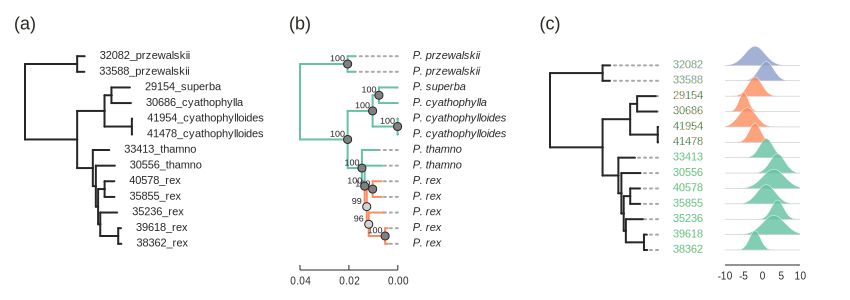
\includegraphics[width=.99\textwidth]{ToyTree-figure}
    \caption{Example toytree plots. (a) A tree drawing with default styling produced by calling .draw() from a ToyTree object; (b) Extensive styling can be added to trees using values extracted from ToyTrees in the proper order for plotting; (c) The simple layout of \emph{toytree} plots makes it easy to add additional plots on the same coordinate axes using the \emph{toyplot} library. The displayed tree is from \cite{eaton_inferring_2013}. See Appendix for the full code to reproduce these figures.}
\end{figure}


\subsubsection*{TreeNodes and Toytrees}
\emph{Toytree} uses a forked and modified version of the TreeNode class object from the \emph{ete3} library \citep{huerta-cepas_ete_2016} to represent nodes in a tree. A tree is represented by a collection of TreeNodes with pointers designating ancestor and descendant relationships. Each TreeNode has a default set of features (name, dist, support, height, idx) that can be modified or added to by users. 
In \emph{toytree} TreeNodes are nested within a ToyTree object, and thus most users will not interact with TreeNodes directly. TreeNodes represent individual nodes, and ToyTrees represent the collection of TreeNodes, with attributes and functions at that level. ToyTrees store plotting coordinates that are updated whenever trees are modified; provide user-friendly functions for modifying trees; and provide functions for accessing attributes of trees, such as node values or tip labels \textcolor{black}{that can be used to extract values in node plot order to easily modify node styles (e.g., size, color) based on attribute values. Tree modification functions of Toytrees are largely based on ete3 functions but sync with plotting coordinates, return copies instead of operating in-place to allow for chaining multiple functions together, and allow selecting clades or tips based on fuzzy label matching, simple expressions, or common ancestor relationships.}


\subsubsection*{Reproducible and robust workflows}
A challenge when working with trees and tree drawings is to ensure that the correct values (e.g., names or support values) are plotted on the correct nodes or edges of the tree, and that these remain associated throughout manipulations of the tree, such as collapsing or rotating nodes, modifying names, or re-rooting. %It has been shown previously that many tree visualization tools mismanage node values when trees are rerooted \citep{czech_critical_2017}. Toytree does not suffer this error, and aims to reduce similar errors by providing 
\textcolor{black}{Toytree aims to reduce errors that come from improperly aligning node or tip data with a tree structure once it is modified by providing functions for extracting data directly from ToyTree objects}. This approach ensures the data are returned in the order in which they will be plotted (Fig.~2). Mistakes can be further avoided by using the style argument node\_hover=True, which activates an interactive hover feature to show all attributes of nodes when hovered over by a cursor. This allows one to easily check that node names, supports, and edge lengths are coordinated, and to explore multiple node features at once.


\begin{figure}
  \centering
  \includegraphics[width=.99\textwidth]{code-cells-1}
  \caption{The function .get\_node\_values() extracts data from ToyTree objects in the order it will be plotted. Style arguments can be supplied as a single value that will apply to all features, or as a list of values that will apply to each feature individually. This example shows simple Python code to construct one list of values for applying node colors to nodes based on their support values. The effect of these styling options can be seen in Fig.~1a and Fig.~1b.
}
\end{figure}


\subsubsection*{Utility functions}
\emph{Toytree} includes functions to generate random trees in the .rtree submodule, and to modify trees in the .mod submodule. The .rtree functions can generate trees that are balanced or imbalanced, with equal or random branch lengths, and as coalescent trees. The .mod functions can be used to scale node heights by a constant, randomly slide node heights, or to make trees ultrametric. These simple functions can be generally useful for generating trees for comparing the effects of tree shape and edge lengths when testing evolutionary hypotheses. 

\subsubsection*{Multitree objects}
Multiple trees can be parsed and stored together in the MultiTree class object to coordinate comparing and plotting sets of trees. Two MultiTree plotting functions are currently available: .draw\_tree\_grid() and .draw\_cloud\_tree(). The first arranges multiple trees on a coordinate grid, while the latter plots overlapping trees on the same coordinate axes (Fig.~3). Cloud trees are primarily used to visualize discordance among topologies, which is most easily observed when overlapping trees are plotted with a fixed order of the tips. In tree grid drawings users can also optionally fix the order of tips to better visualize discordance (Fig.~3A-B). For both types of plots, the style of individual trees can be modified as well, as in Fig.~3C, where different edge colors are applied to trees that match or do not match the majority-rule consensus topology. Programmatic drawing of cloud trees makes it possible to generate complex plots using very simple code (Fig. 3D; Fig.~4). Finally, MultiTree objects can return a majority-rule consensus tree from a set of trees and calculate support values for splits in the tree. 

\begin{figure}
  \centering
    \includegraphics[width=.75\textwidth]{MultiTree-figure}
    \caption{MultiTree class objects can be used to parse, store, compare, and plot sets of trees. (a) A tree grid plot is a simple function for displaying multiple trees on a grid. (b) The same tree grid plot with the fixed\_order=True argument; it is easy to observe differences among trees by fixing the tip order. (c) A cloud tree plot shows multiple trees overlapping with a fixed tip order. Different styles can be applied to each tree; here topologies matching the majority-rule consensus are in orange, while those not matching are in blue. (d) Extensive styling can be applied to cloud trees: this example reproduces a cloud tree from \cite{cui_phylogenomics_2013} using \emph{toytree}. See Appendix for the full code to reproduce figures.}
\end{figure}

\begin{figure}
  \centering
    \includegraphics[width=.99\textwidth]{code-cells-2}
\caption{Example code to generate MultiTree drawings from sets of trees as shown in Fig.~3.}
\end{figure}

\subsubsection*{Conclusions}
\emph{Toytree} is a simple but powerful tree plotting library for Python. It provides pleasant out-of-the-box styling for displaying trees, simple methods for manipulating them, and is easy to install and use. It can integrate easily with existing Python tree analysis packages. Future developments will include support for circular tree layouts, faster rendering of trees by simplifying CSS code, additional tree modification functions, and integration with other Python and R libraries for plotting results of comparative analyses on trees.


\subsubsection*{Acknowledgements}
During the development of toytree I received support from the National Science Foundation grant DEB-1557059 and Columbia University startup funds. I would like to thank Timothy Shead for helpful advice and for motivating the development of this software. 


\subsubsection*{Data Availability}
Toytree source code is available at \url{https://github.com/eaton-lab/toytree} with the current version 1.0.0 archived at DOI: \url{10.5281/zenodo.3445526}. A jupyter notebook to reproduce figures in this publication is available in the supplementary materials and on GitHub: \url{https://nbviewer.jupyter.org/github/eaton-lab/toytree/tree/master/manuscript/}

\clearpage
\newpage


\begin{thebibliography}{16}
\expandafter\ifx\csname natexlab\endcsname\relax\def\natexlab#1{#1}\fi

\bibitem[{Baum \emph{et~al.}(2005)Baum, Smith \&
  Donovan}]{baum_tree-thinking_2005}
Baum, D.A., Smith, S.D. \& Donovan, S.S.S. (2005).
\newblock The {Tree}-{Thinking} {Challenge}.
\newblock \emph{Science}, 310, 979--980.

\bibitem[{Cui \emph{et~al.}(2013)Cui, Schumer, Kruesi, Walter, Andolfatto \&
  Rosenthal}]{cui_phylogenomics_2013}
Cui, R., Schumer, M., Kruesi, K., Walter, R., Andolfatto, P. \& Rosenthal, G.G.
  (2013).
\newblock Phylogenomics {Reveals} {Extensive} {Reticulate} {Evolution} in
  {Xiphophorus} {Fishes}.
\newblock \emph{Evolution}, 67, 2166--2179.

\bibitem[{Eaton \& Ree(2013)}]{eaton_inferring_2013}
Eaton, D.A.R. \& Ree, R.H. (2013).
\newblock Inferring {Phylogeny} and {Introgression} using {RADseq} {Data}: {An}
  {Example} from {Flowering} {Plants} ({Pedicularis}: {Orobanchaceae}).
\newblock \emph{Systematic Biology}, 62, 689--706.

\bibitem[{Harmon \emph{et~al.}(2008)Harmon, Weir, Brock, Glor \&
  Challenger}]{harmon_geiger:_2008}
Harmon, L.J., Weir, J.T., Brock, C.D., Glor, R.E. \& Challenger, W. (2008).
\newblock {GEIGER}: investigating evolutionary radiations.
\newblock \emph{Bioinformatics}, 24, 129--131.

\bibitem[{Huerta-Cepas \emph{et~al.}(2016)Huerta-Cepas, Serra \&
  Bork}]{huerta-cepas_ete_2016}
Huerta-Cepas, J., Serra, F. \& Bork, P. (2016).
\newblock {ETE} 3: {Reconstruction}, {Analysis}, and {Visualization} of
  {Phylogenomic} {Data}.
\newblock \emph{Molecular Biology and Evolution}, 33, 1635--1638.

\bibitem[{Kluyver \emph{et~al.}(2016)Kluyver, Ragan-Kelley, Pérez, Granger,
  Bussonnier, Frederic, Kelley, Hamrick, Grout, Corlay, Ivanov, Avila, Abdalla,
  Willing \& al}]{kluyver_jupyter_2016}
Kluyver, T., Ragan-Kelley, B., Pérez, F., Granger, B.E., Bussonnier, M.,
  Frederic, J., Kelley, K., Hamrick, J.B., Grout, J., Corlay, S., Ivanov, P.,
  Avila, D., Abdalla, S., Willing, C. \& al, e. (2016).
\newblock Jupyter {Notebooks} - a publishing format for reproducible
  computational workflows.
\newblock In: \emph{{ELPUB}}.

\bibitem[{Oliphant(2015)}]{oliphant_guide_2015}
Oliphant, T.E. (2015).
\newblock \emph{Guide to {NumPy}}.
\newblock 2nd edn.
\newblock CreateSpace Independent Publishing Platform, USA.

\bibitem[{Paradis \emph{et~al.}(2004)Paradis, Claude \&
  Strimmer}]{paradis_ape:_2004}
Paradis, E., Claude, J. \& Strimmer, K. (2004).
\newblock {APE}: {Analyses} of {Phylogenetics} and {Evolution} in {R} language.
\newblock \emph{Bioinformatics}, 20, 289--290.

\bibitem[{Paradis \& Schliep(2019)}]{paradis_ape_2019}
Paradis, E. \& Schliep, K. (2019).
\newblock ape 5.0: an environment for modern phylogenetics and evolutionary
  analyses in {R}.
\newblock \emph{Bioinformatics}, 35, 526--528.

\bibitem[{Pedregosa \emph{et~al.}(2011)Pedregosa, Varoquaux, Gramfort, Michel,
  Thirion, Grisel, Blondel, Prettenhofer, Weiss, Dubourg, Vanderplas, Passos,
  Cournapeau, Brucher, Perrot \& Duchesnay}]{pedregosa_scikit-learn:_2011}
Pedregosa, F., Varoquaux, G., Gramfort, A., Michel, V., Thirion, B., Grisel,
  O., Blondel, M., Prettenhofer, P., Weiss, R., Dubourg, V., Vanderplas, J.,
  Passos, A., Cournapeau, D., Brucher, M., Perrot, M. \& Duchesnay, �. (2011).
\newblock Scikit-learn: {Machine} {Learning} in {Python}.
\newblock \emph{Journal of Machine Learning Research}, 12, 2825−2830.

\bibitem[{Perez \& Granger(2007)}]{perez_ipython:_2007}
Perez, F. \& Granger, B.E. (2007).
\newblock {IPython}: {A} {System} for {Interactive} {Scientific} {Computing}.
\newblock \emph{Computing in Science \& Engineering}, 9, 21--29.

\bibitem[{Rambaut(2010)}]{rambaut_figtree_2010}
Rambaut, A. (2010).
\newblock {FigTree} v1.3.1.

\bibitem[{Revell(2012)}]{revell_phytools:_2012}
Revell, L.J. (2012).
\newblock phytools: an {R} package for phylogenetic comparative biology (and
  other things).
\newblock \emph{Methods in Ecology and Evolution}, 3, 217--223.

\bibitem[{Shead(2014)}]{shead_toyplot_2014}
Shead, T.M. (2014).
\newblock toyplot.
\newblock Tech. Rep. TOYPLOT; 003233MLTPL00, Sandia National Laboratory.

\bibitem[{Sukumaran \& Holder(2010)}]{sukumaran_dendropy:_2010}
Sukumaran, J. \& Holder, M.T. (2010).
\newblock {DendroPy}: a {Python} library for phylogenetic computing.
\newblock \emph{Bioinformatics}, 26, 1569--1571.

\bibitem[{Talevich \emph{et~al.}(2012)Talevich, Invergo, Cock \&
  Chapman}]{talevich_bio.phylo:_2012}
Talevich, E., Invergo, B.M., Cock, P.J. \& Chapman, B.A. (2012).
\newblock Bio.{Phylo}: {A} unified toolkit for processing, analyzing and
  visualizing phylogenetic trees in {Biopython}.
\newblock \emph{BMC Bioinformatics}, 13, 209.

\end{thebibliography}


% \bibliography{revision}
\bibliographystyle{ecol_let}

\end{document}
